\renewcommand{\FileName}{nway2}

% these two frames covered in mosbasic
\begin{comment}
\begin{frame}
%\makeatletter\slidebox@restore\makeatother
\frametitle{Mosaic displays and Log-linear Models}
\citet{HartiganKleiner:81,Friendly:94a,Friendly:99b}:
\begin{itemize}
\item \boldital{Width} $\sim$ one set of marginals, $n_{i+}$
\item \boldital{Height} $\sim$ relative proportions of other variable, 
$p_{j\given i} = n_{ij} / n_{i+}$
\item $\Rightarrow$ \textbf{area} $\sim$ \textbf{frequency}, $n_{ij} = n_{i+} p_{j\given i}$
\begin{center}
  \includegraphics[width=.5\dispwidth,clip]{fig/mosaic9a1f}
\end{center}
\end{itemize}
\end{frame}

\begin{frame}
\begin{itemize}
\item \boldital{Shading}: Sign and magnitude of Pearson
$\chi^2$ residual,
$d_{ij} = ( n_{ij} - \hat{m}_{ij} ) / \sqrt{\hat{m}_{ij}}$ (or L.R. $G^2$)
\begin{itemize*}
\item Sign: \red{$-$ negative in red}; \blue{$+$ positive in blue}\black
\item Magnitude: intensity of shading:  $|d_{ij}| > 0, 2, 4, \dots$
\end{itemize*}
\item \boldital{Independence}: Rows $\approx$ align, \emph{or}
cells are empty!
\item E.g., aggregate Berkeley data, independence model:
\end{itemize}

\begin{center}
  \includegraphics[width=.5\dispwidth,clip]{fig/mosaic9a1f}
\end{center}
\end{frame}
\end{comment}

\begin{frame}
  \frametitle{Mosaic displays: Hair color and eye color}
  \vspace{2ex}
 \begin{minipage}[c]{.49\dispwidth}
  \includegraphics[width=1\linewidth,clip]{fig/mosaic3m1}
 \end{minipage}%
 \hfill
 \begin{minipage}[c]{.49\dispwidth}
  We know that hair color and eye color are associated ($\chi^2 (9) = 138.29$).
  The question is \alert{how}?
  \begin{itemize}
  \item Dark hair goes with dark eyes, light hair with light eyes
  \item Red hair, hazel eyes an exception?
  \item Effect ordering: Rows/cols permuted by CA Dimension 1
  \item[$\Rightarrow$] Opposite corner pattern
  \end{itemize}
 \end{minipage}
\end{frame}

\begin{frame}
\frametitle{Mosaic displays: Marginal models}
Berkeley data: Departments $\times$ Gender (ignoring Admit):
\begin{itemize}
\item Did departments differ in the total number of applicants?
\item Did men and women apply differentially to departments?
%\item Model [Dept] [Gender]: $G^2_{(5)} =$ 1220.6.
\end{itemize}

 \begin{minipage}[c]{.49\dispwidth}
  \includegraphics[width=1\linewidth,clip]{fig/mosaic9a2f}
 \end{minipage}%
 \hfill
 \begin{minipage}[c]{.49\dispwidth}
\begin{itemize*}
\item Model [Dept] [Gender]: $G^2_{(5)} =$ 1220.6.
\item \boldital{Note}: Departments ordered A--F by overall rate of admission.
\end{itemize*}
 \end{minipage}
	
\end{frame}

\begin{frame}
\frametitle{Mosaic displays for multiway tables}
\begin{itemize}
\item Generalizes to $n$-way tables: divide cells recursively
\item Can fit \emph{any} log-linear model (e.g., 2-way, 3-way, $\dots$),
	\begin{itemize*}
	\item For a 3-way table:  [A][B][C], [AB][C], [AB][AC], $\dots$, [ABC]
	\end{itemize*}

%\scalebox{.9}{%
%\input{tab/loglin-3way}
%}

%e.g., the model for conditional independence ($A \perp C \given B$):
%\begin{equation*}
%[AB][BC] \equiv
%  \log \,  m_{ijk}  =
%  \mu
%  +  \lambda_i^A
%  +  \lambda_j^B
%  +  \lambda_k^C
%  +  \lambda_{ij}^{AB}
%  +  \lambda_{jk}^{BC}
%\end{equation*}

\item Each mosaics shows:
	\begin{itemize*}
	\item  \alert{\textbf{DATA}} (size of tiles)
	\item (some) \alert{\textbf{marginal}} frequencies (spacing $\rightarrow$ visual grouping)
	\item  \alert{\textbf{RESIDUALS}} (shading) --- what associations have been omitted?
	\end{itemize*}
\item Visual fitting:
	\begin{itemize*}
	\item Pattern of lack-of-fit (residuals) $\rightarrow$ ``better'' model---
	smaller residuals 
	\item ``cleaning the mosaic'' $\rightarrow$ ``better'' model---
	empty cells
	\item best done interactively!
	\end{itemize*}
\end{itemize}

\end{frame}

\begin{frame}
\begin{itemize}
\item E.g., Joint independence, [DG][A] (null model, Admit as response)
[$G^2_{(11)}$ = 877.1]:
\end{itemize}
\begin{center}
  \includegraphics[width=.55\dispwidth,clip]{fig/mosaic9a3f}
\end{center}
\end{frame}

\begin{frame}
%\makeatletter\slidebox@restore\makeatother
%\iflandscape\def\dispfactor{.5}\else \def\dispfactor{.7}\fi
\frametitle{Mosaic displays for multiway tables}
\begin{itemize}
\item Visual fitting:
%	\begin{itemize*}
%	\item Pattern of lack-of-fit (residuals) $\rightarrow$ ``better'' model---
%	smaller residuals 
%	\item ``cleaning the mosaic'' $\rightarrow$ ``better'' model---
%	empty cells
%	\item best done interactively!
%	\end{itemize*}
\end{itemize}

 \begin{minipage}[c]{.55\dispwidth}
  \includegraphics[width=1\linewidth,clip]{fig/mosaic9a4f}
 \end{minipage}%
 \hfill
 \begin{minipage}[c]{.44\dispwidth}
  \begin{itemize}
  \item E.g., Add [Dept Admit] association $\rightarrow$ Conditional independence: 
   \begin{itemize*}
   \item Fits poorly: ($G^2_{(6)}$ = 21.74)
   \item But, only in Department A!
   \end{itemize*}
   \item The GLM approach allows fitting a special term for Dept. A
   \item Technical note:  These displays use \emph{standardized residuals}: better
    statistical properties. 
  \end{itemize}
 \end{minipage}
\end{frame}

\begin{frame}
  \frametitle{Other variations: Double decker plots}
	 \begin{itemize*}
		 \item Visualize dependence of one categorical (typically binary) variable on predictors
		 \item Formally: mosaic plots with vertical splits for all \alert{predictor dimensions}, highlighting the
		 response by shading
	 \end{itemize*}
 \begin{center}
%	\setkeys{Gin}{width=.75\textwidth}
\includegraphics[width=.75\textwidth]{fig/plt-UCB-doubledecker}
 \end{center}
\end{frame}


\subsection{Sequential plots and models}
\begin{frame}
  \frametitle{Sequential plots and models}
  \begin{itemize}
	\item Mosaic for an \nway\ table $\rightarrow$ hierarchical decomposition of association in a way
analogous to \alert{sequential fitting} in regression
    \item Joint cell probabilities are decomposed as
\begin{equation*}
p_{ijk\ell \cdots} = \underbrace{\overbrace{p_i \times p_{j|i}}^{\{v_1 v_2\}} \times \: p_{k|ij}}_{\{v_1 v_2 v_3\}}
       \times \: p_{\ell|ijk} \times\cdots \times p_{n|ijk\cdots}
\end{equation*}
	
      \begin{itemize*}
	  \item First 2 terms $\rightarrow$ mosaic for $v_1$ and $v_2$
	  \item First 3 terms $\rightarrow$ mosaic for $v_1$, $v_2$ and $v_3$
	  \item $\cdots$
	  \end{itemize*}
	\item Sequential models of \emph{joint independence} $\rightarrow$
	additive decomposition of the total association,
	$G^2_{[v_1] [v_2] \dots [v_p]}$ (mutual independence),
\begin{equation*}
G^2_{[v_1] [v_2] \dots [v_p]} =
G^2_{[v_1] [v_2]} +
G^2_{[v_1 v_2] [v_3]} +
G^2_{[v_1 v_2 v_3] [v_4]} + \cdots+
G^2_{[v_1 \dots v_{p-1}] [v_p]}
\end{equation*}
   \item As in regression, most useful when there is some \alert{substantive ordering} of the variables
 \end{itemize}

\end{frame}

\begin{frame}
   \frametitle{Sequential plots and models: Example}
%\iflandscape\def\dispfactor{.65}\else \def\dispfactor{.7}\fi
  \begin{itemize}
    \item Hair color x Eye color marginal table (ignoring Sex)
  \end{itemize}
\begin{center}
  \includegraphics[width=.6\dispwidth,clip]{fig/mosaic3mj2}
\end{center}
   
\end{frame}

\begin{frame}
   \frametitle{Sequential plots and models: Example}
  \begin{itemize}
    \item 3-way table, Joint Independence Model [Hair Eye] [Sex]
  \end{itemize}
\begin{center}
  \includegraphics[width=.6\dispwidth,clip]{fig/mosaic3mj3}
\end{center}
   
\end{frame}

\begin{frame}
   \frametitle{Sequential plots and models: Example}
  \begin{itemize}
    \item 3-way table, Mutual Independence Model [Hair] [Eye] [Sex]
  \end{itemize}
\begin{center}
  \includegraphics[width=.6\dispwidth,clip]{fig/mosaic3mj1}
\end{center}
   
\end{frame}

\begin{frame}
   \frametitle{Sequential plots and models: Example}
%% three subfig side-by-side
 \begin{minipage}[c]{.3\textwidth}
  \centering Marginal 
  \\ \includegraphics[width=1\linewidth,clip]{fig/mosaic3mj2}
  \\ \centering [Hair] [Eye]
  \\ \centering $G^2_{(9)} = 146.44$
 \end{minipage}%
 \hfill {\Large +} \hfill
 \begin{minipage}[c]{.3\textwidth}
  \centering Joint 
  \\ \includegraphics[width=1\linewidth,clip]{fig/mosaic3mj3}
  \\ \centering [Hair Eye] [Sex]
  \\ \centering $G^2_{(15)} = 19.86$
 \end{minipage}
 \hfill {\Large =} \hfill
 \begin{minipage}[c]{.3\textwidth}
  \centering Total 
  \\ \includegraphics[width=1\linewidth,clip]{fig/mosaic3mj1}
  \\ \centering [Hair] [Eye] [Sex]
  \\ \centering $G^2_{(24)} = 166.30$
 \end{minipage}
 
\end{frame}

% slide template
\subsection{Mosaic matrices}
\begin{frame}
  \frametitle{Mosaic matrices}
  \begin{itemize}
	\item Analog of \emph{scatterplot matrix} for categorical data \citep{Friendly:99b}
      \begin{itemize*}
	  \item Shows all $p (p-1)$ pairwise views in a coherent display
	  \item Each pairwise mosaic shows bivariate (marginal) relation
	  \item Fit: marginal independence
	  \item Residuals: show \alert{marginal} associations
	  \item Direct visualization of the ``Burt'' matrix analyzed in
	  MCA for $p$ categorical variables
	  \end{itemize*}
  \end{itemize}
\begin{center}
  \includegraphics[width=.4\dispwidth,clip]{fig/mosmat3}
\end{center}
\end{frame}

\begin{frame}
  Hair, Eye, Sex data:
\begin{center}
  \includegraphics[height=.94\textheight,clip]{fig/mosmat3}
\end{center}
\end{frame}

\begin{frame}
Berkeley data: %(does not display)
\begin{center}
  \includegraphics[height=.94\textheight,clip]{fig/mosmat9m}
\end{center}
\end{frame}

\subsection{Partial association}
\begin{frame}
  \frametitle{Partial association, Partial mosaics}
  \begin{itemize}
	\item{\large\bfseries Stratified analysis:}
      \begin{itemize*}
	  \item How does the association between two (or more) variables vary 
	  over levels of other variables?
	  \item Mosaic plots for the main variables show \emph{partial association}
	  at each level of the other variables.
%	  \item Analog of \emph{coplot} (conditioning plot) for categorical data
	  \item E.g., Hair color, Eye color \emph{BY} Sex $\leftrightarrow$ 
	  \texttt{TABLES sex * hair * eye;}
      \end{itemize*}
  \end{itemize}
\begin{center}
  \includegraphics[width=.86\dispwidth,clip]{fig/mospart3}
\end{center}

\end{frame}

\begin{frame}

  \frametitle{Partial association, Partial mosaics}
  \begin{block}{\large\bfseries Stratified analysis: conditional decomposition of $G^2$}
      \begin{itemize*}
	  \item Fit models of partial (conditional) independence, $ A \perp B \given C_k$
            at each level of (controlling for) $C$.
	  \item $\Rightarrow$ partial $G^2$s add to the overall
	  $G^2$ for conditional independence,$ A \perp B \given C$
\begin{equation*}
G^2_{A \perp B \given C} = \sum_k G^2_{A \perp B \given C(k)}
\end{equation*}
       \end{itemize*}
 \end{block}

\input{tab/haireyesex}
\end{frame}


%\input{frames/dummy}

\endinput

% two figures 
 \begin{minipage}[b]{.5\linewidth}
  \centering
  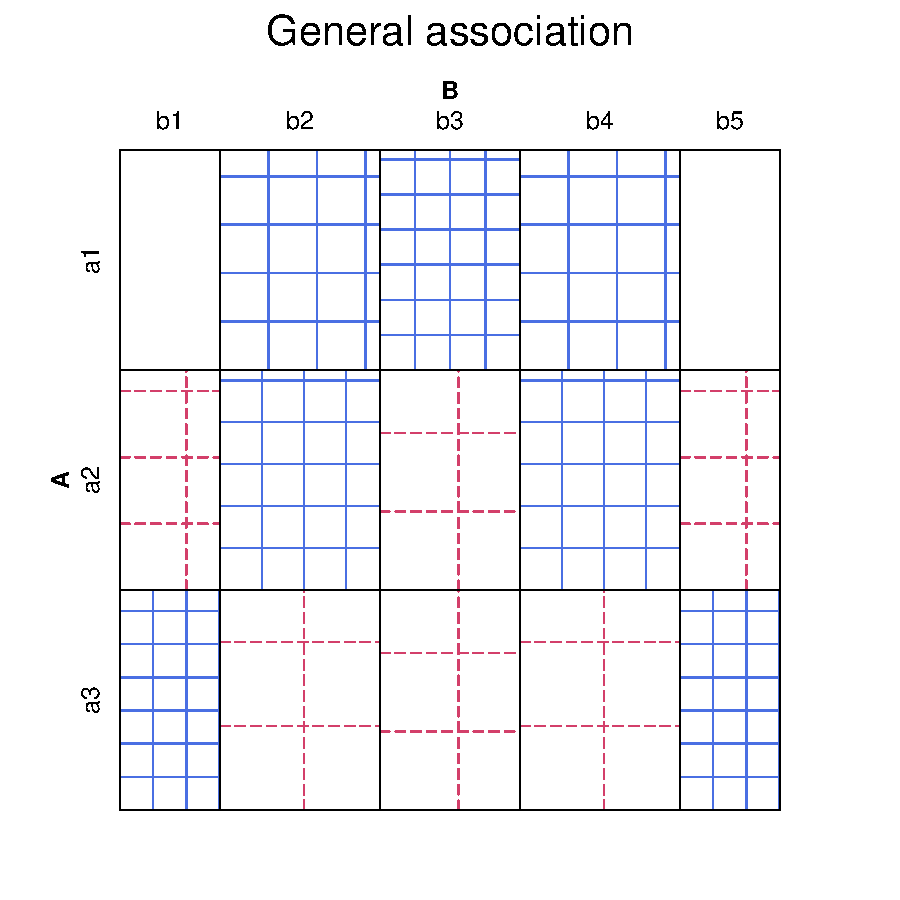
\includegraphics[width=.95\linewidth]{fig/cmhdemo1}
 \end{minipage}%
 \begin{minipage}[b]{.5\linewidth}
  \centering
  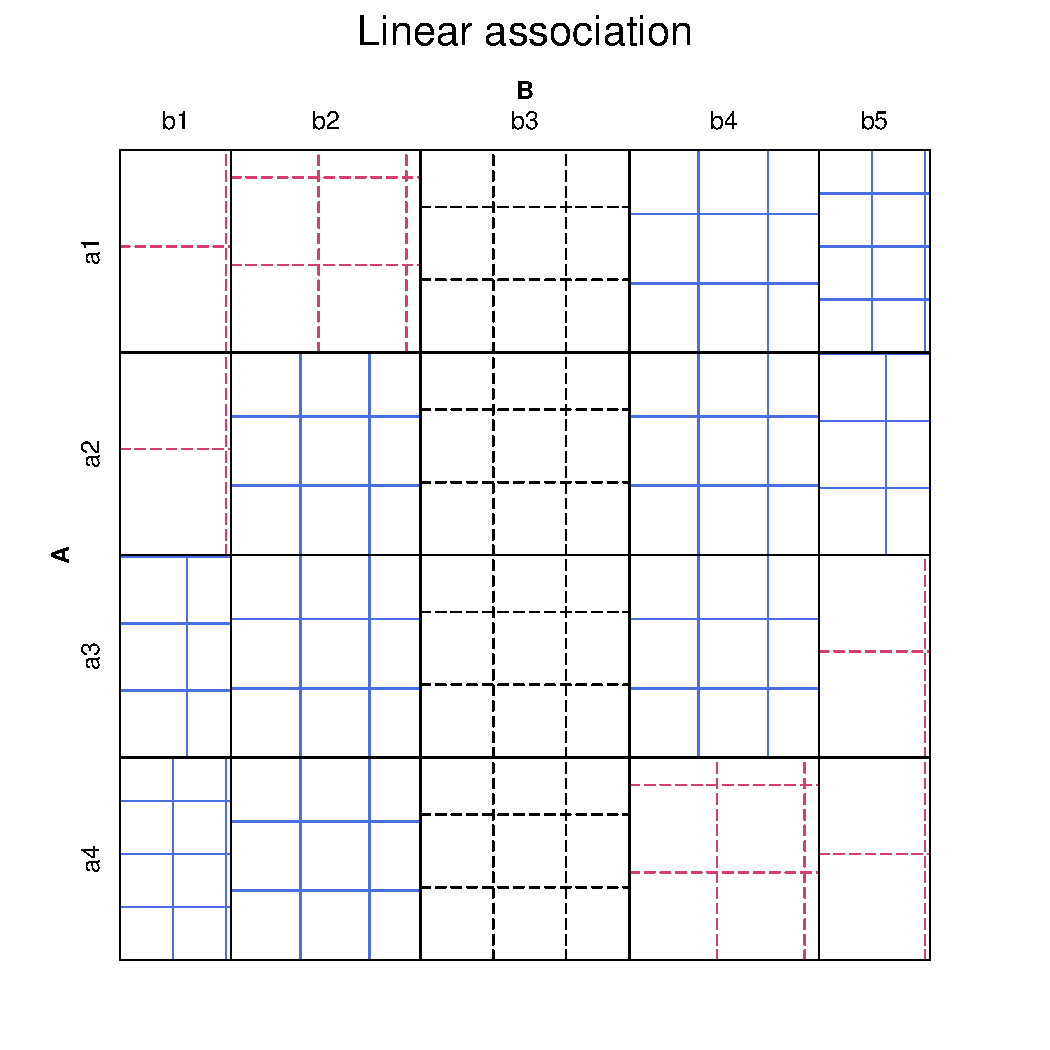
\includegraphics[width=.95\linewidth]{fig/cmhdemo2}
 \end{minipage}

% slide template
\begin{frame}
  \frametitle{}
  \begin{itemize}
	\item{\large\bfseries }
      \begin{itemize*}
	  \item 
    	\begin{itemize*}
		\item 
		\item 
		\end{itemize*}
	  \item 
	  \end{itemize*}
	\item{\large\bfseries }
	\item{\large\bfseries }
  \end{itemize}
\end{frame}

